\section{Τεχνολογική Στοίβα}
\begin{frame}
	\frametitle{Τεχνολογική Στοίβα}
	\centering
	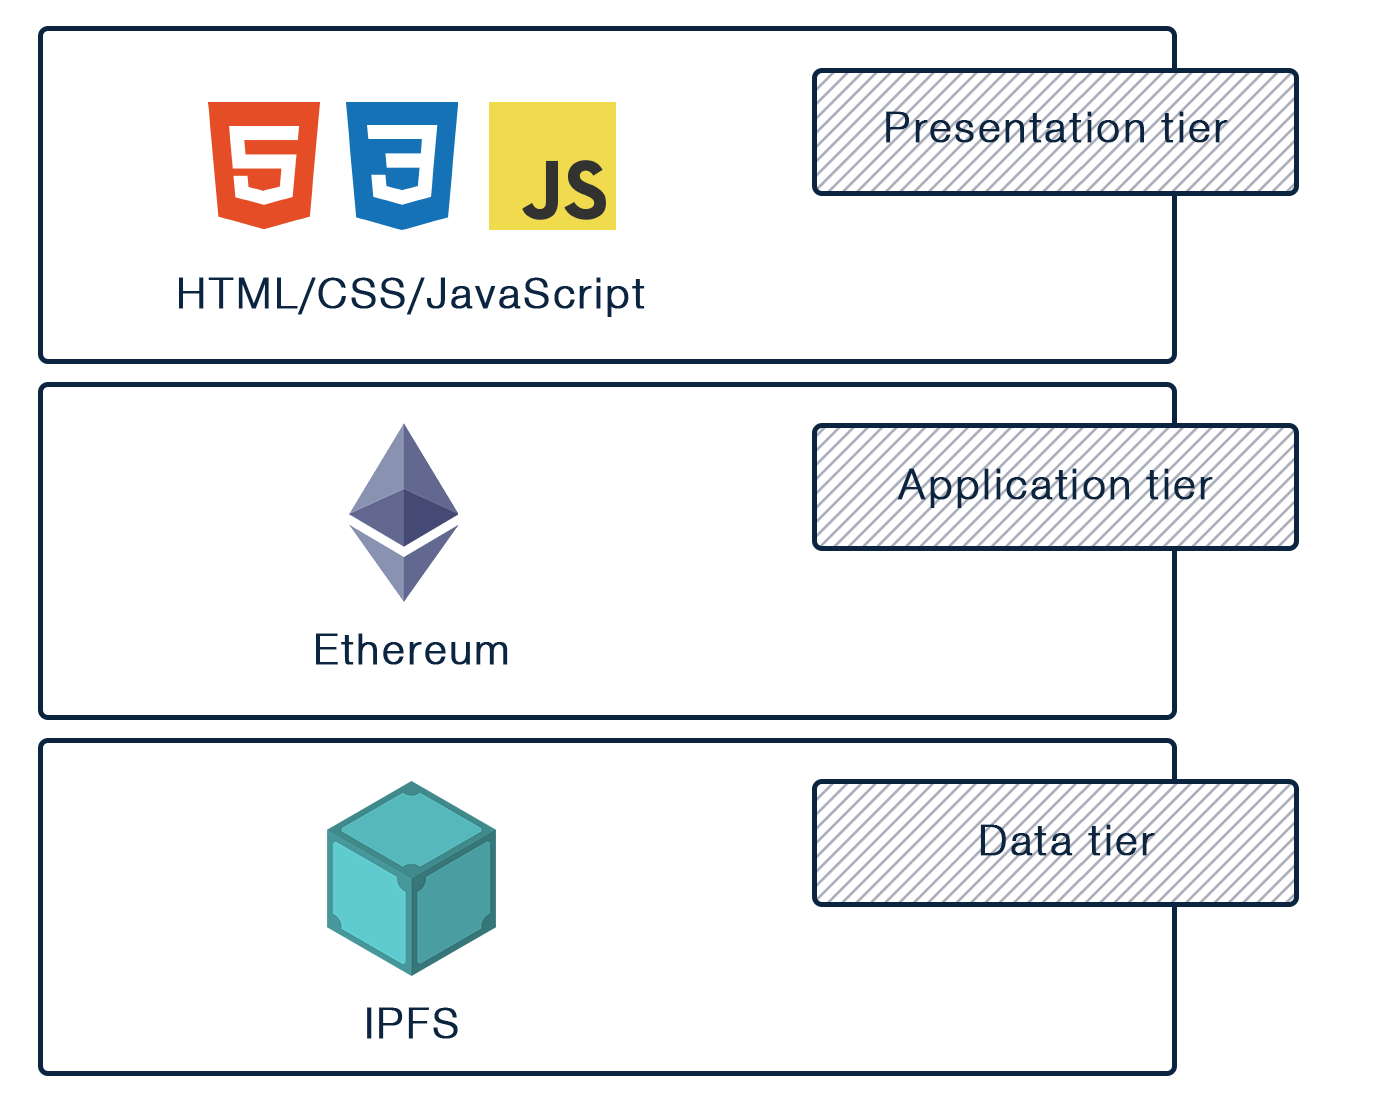
\includegraphics[scale=0.15]{assets/figures/technology-stack}
\end{frame}

\note{
	Ξεκινώντας τη σχεδίαση της πλατφόρμας, πραγματοποιήσαμε έρευνα για την επιλογή της τεχνολογικής στοίβας. Αυτή αποφασίσαμε να ακολουθήσει μία προσαρμοσμένη για τα δεδομένα μορφή τριμερούς διάταξης και έτσι να χωριστεί σε τρία λογικά επίπεδα, όπως φαίνονται στη διαφάνεια.
	Το πρώτο επίπεδο, δηλαδή το Presentation tier, αποτελεί τη διεπαφή του χρήστη, μέσω της οποίας εκείνος αλληλεπιδρά με την εφαρμογή. Αυτό αναπτύχθηκε ως μία κλασική client-side web application σε HTML/CSS/JavaScript με τη χρήση σύγχρονων web framework και δε θα το αναλύσουμε ιδιαίτερα.
	Το δεύτερο επίπεδο, δηλαδή το Application tier, είναι εκείνο στο οποίο πραγματοποιείται η επεξεργασία της εφαρμογής. Εδώ επιλέξαμε να χρησιμοποιήσουμε το blockchain και τα smart contract και συγκεκριμένα την πλατφόρμα του Ethereum.
	Τέλος, για το τρίτο επίπεδο, δηλαδή το Data tier, το οποίο είναι υπεύθυνο για την αποθήκευση του κύριου όγκου των δεδομένων, επιλέχθηκε το IPFS.
}
